\authoredsubsection{Sprint 5}{Sebastian}{Sebastian Straub}\label{sec:sprint5}

Sprint 5 ran from 23 June to 06 July 2026, with the review and retrospective held on 07 July, and closed the project. With the pipeline fully integrated at the end of Sprint 4, the character of the work changed. The focus shifted from building new capability toward proving the self-improvement loop end to end, making its performance visible to operators, and handing the system over to Interhyp in a state the team could walk away from. Sebastian Straub served as Scrum Master for this final sprint.

\subsubsection{Sprint Goals}\label{sec:sprint5-goals}

The sprint goal committed the team to running systematic batch evaluations of the full pipeline against the ground-truth test dataset, building a Batch-Running Dashboard and an Optimization Dashboard to make routing accuracy and optimization cycles visible, deploying the system, and preparing the final presentation, the handover document, and a knowledge transfer session for Interhyp. Behind these deliverables stood one measurable outcome, defined as Interhyp being able to operate, evaluate, and extend the pipeline independently by the end of the sprint. The goal was deliberately phrased around this outcome, since a final sprint that leaves a working yet unexplainable system behind would have missed the point of the engagement.

\subsubsection{Sprint Planning}\label{sec:sprint5-planning}

Planning started from two gaps left open after Sprint 4. The optimizer's execution flow was not yet visible in the frontend, and no dedicated view measured routing accuracy over time, which Interhyp had explicitly requested during the Sprint 4 review. The resulting backlog contained seven tickets totaling 25 story points, consistent with the velocity established over the previous sprints. The stand-up cadence of four meetings per week was kept unchanged, with the in-person Tuesday session continuing to anchor each week ahead of the Interhyp meeting.

\Cref{fig:sprint5-backlog} shows the resulting backlog. The Batch-Running Dashboard (five story points) lay with Sebastian Straub, the Optimization Dashboard (three) with Gáspár Harmati supported by Sebastian Straub, the Monitoring Dashboard (three) with Marco Schröder, System Deployment (five) with Julius Bethge, the Handover Document (two) with Gáspár Harmati, and the Knowledge Transfer Session (two) with Mohsin Saeed. The Final Presentation (five) was split into one subtask per team member and coordinated by Mohsin Saeed, since it had to bring the work of all five into one consistent story.

\begin{figure}
\centering
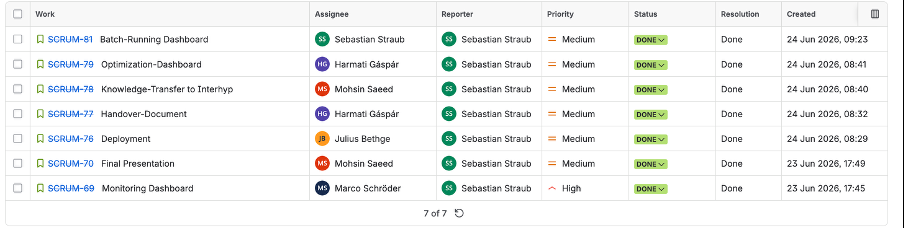
\includegraphics[width=1\linewidth,height=\textheight,keepaspectratio]{assets/sprints/sprint5-backlog.png}
\caption{Sprint 5 backlog showing owners and completion status (Jira).}\label{fig:sprint5-backlog}
\end{figure}

\subsubsection{Implementation and Execution}\label{sec:sprint5-execution}

The sprint delivered three operator-facing dashboards on top of the existing chat and pipeline views. The Training Dashboard produces the labeled data the optimizer learns from. It runs an uploaded dataset through the full router, has the LLM judge score every routing decision, and reports accuracy, Stage 1 share, and cost per run. The Evaluation Dashboard measures a prompt version against a fixed held-out dataset and compares two versions side by side, down to a per-agent breakdown, a confusion matrix, and a diff of the exact prompt text that changed. The Optimization Dashboard makes the OPRO loop watchable in real time, plotting the score of every candidate prompt in every round. The Monitoring Dashboard complements them with an operations view of query volume, cost, Stage 1 share, and per-agent accuracy over time. All views stream their data over the same reactive Convex connection that powers the chat, so results appear live without any refresh.

Several operational details determine how these views hold up in day-to-day use. Every training run is preserved as its own record, labeled with the prompt version it ran under, so operators can compare how one dataset performed across prompt versions without re-running anything. Long runs can be stopped from the dashboard, and the worker picks the signal up within a few processed items and terminates cleanly. Evaluation runs skip answer generation entirely, since only the routing decision is measured, which makes each evaluation call faster and cheaper than a full dispatch. The optimization view plots the seed prompt, the best score per round, and every individual candidate, and once a champion prompt is deployed it shows the previous and the new version side by side with the changed lines highlighted. The Monitoring Dashboard is fully wired to the backend but currently displays simulated demo data, since PropDesk has not yet processed real broker traffic, and it will fill with live data without further changes once it does.

The methodologically most important work of the sprint sits beneath these views. Undetected leakage between training and evaluation data is among the most common causes of overoptimistic results in machine-learning-based science \autocite{kapoor2023}, and contaminated benchmarks inflate reported LLM accuracy in the same way \autocite{sainz2023}. The pipeline therefore enforces the separation of training and evaluation data at four independent points. The Training Dashboard strips any prompt that also appears in the evaluation set before an upload reaches the backend, every batch run is tagged as train or eval in the database and filtered at query level, the optimizer's data selector can only ever access training runs, and a server-side guard rejects any attempt to reclassify an evaluation run. This is what allows the Stage 1 thresholds in \cref{sec:router-stage1} to be calibrated on data the reference store has never seen. Without it the accuracy figures in \cref{sec:empirical-evaluation} could not be read as a measurement of routing quality.

Deployment made PropDesk available at a public URL, with sign-in through Google SSO and an email whitelist, and completed the architecture shown in \cref{fig:sprint5-architecture}. A React frontend served from a CDN communicates with Convex, which acts as database, vector store, and job queue at once, while a long-running Python worker polls for jobs and executes the router, judge, and optimizer pipelines. A single environment variable switches the pipeline between a fully local mode, a production mode that routes judge and optimizer through AWS Bedrock in the eu-central-1 region to satisfy Interhyp's EU data residency requirement, and an OpenRouter mode for environments that cannot host models locally.

% Tall, dense diagram: give it a dedicated float page instead of letting it
% claim three quarters of a text page and leave the rest empty.
\begin{figure}[p]
\centering
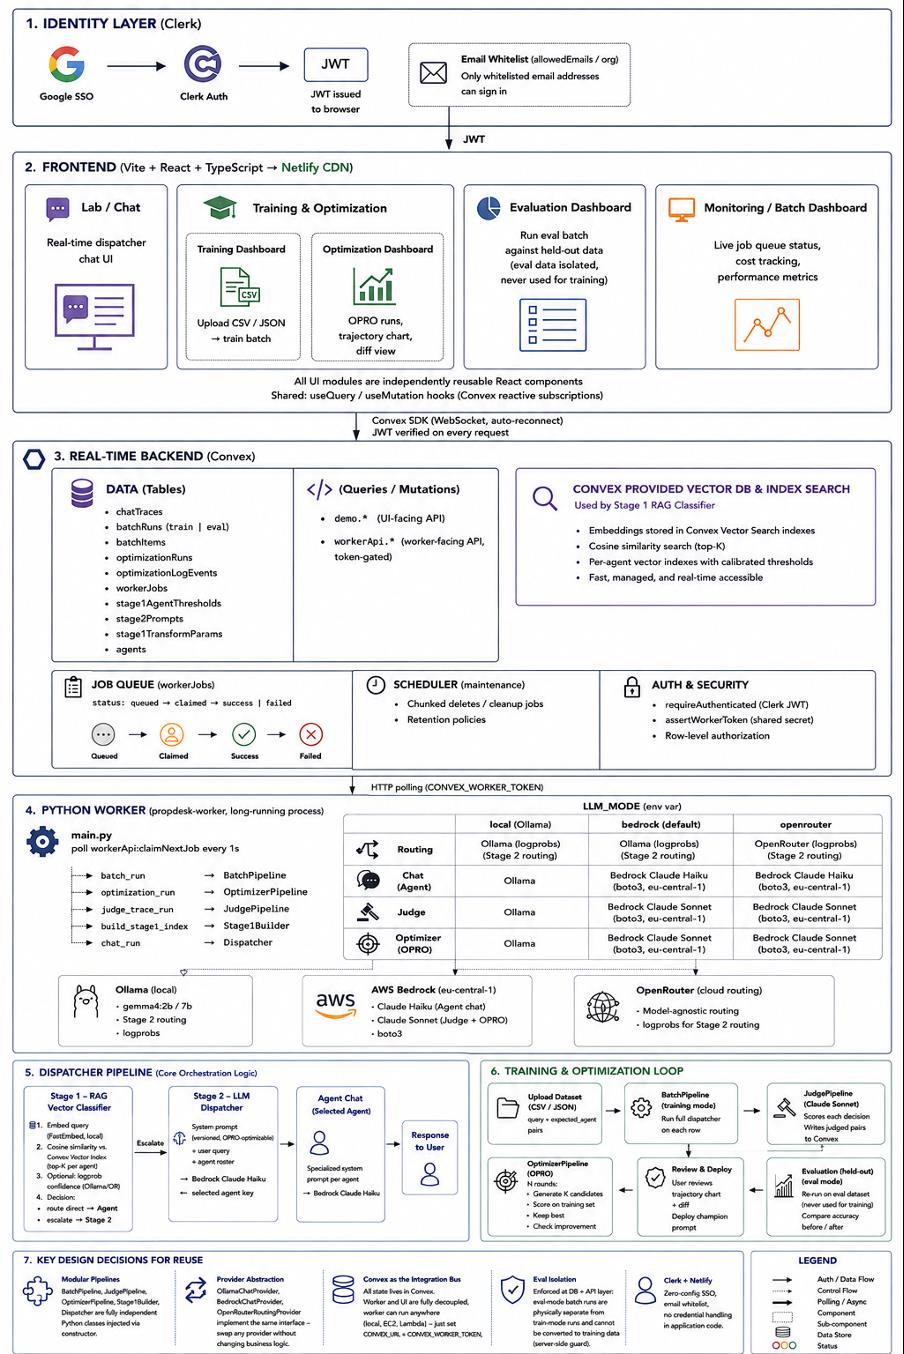
\includegraphics[width=0.95\linewidth,height=0.88\textheight,keepaspectratio]{assets/sprints/sprint5-deployment-architecture.png}
\caption{PropDesk deployment architecture across the identity, frontend, backend, and worker layers (own illustration).}\label{fig:sprint5-architecture}
\end{figure}

A final revision concerned the Stage 1 decision rule. The per-agent margin thresholds from Sprint 3 (\cref{sec:sprint3-execution}) decided escalation on the raw distance between the best and second-best agent score. This worked, but a margin is not comparable across agents and cannot be read as a probability, which made the threshold dashboard hard to interpret and the operating point hard to communicate to Interhyp. Stage 1 was therefore reworked onto a temperature-scaled softmax over the per-agent scores, with the thresholds refitted on the resulting top-agent probability \autocite{guo2017}. Temperature scaling is monotone and cannot alter the agent ranking, so the change affected only the abstention decision. The coverage and risk figures in \cref{sec:router-stage1} are those of the recalibrated configuration and supersede the Sprint 3 values.

The remaining tickets packaged the project for the time after the team. A handover document in C4 style records the architecture together with the decision records behind it, a knowledge transfer session backed by a written operator manual enables Interhyp's data scientists to run the system without the original team, and the final presentation was rebuilt around a simpler narrative after the mid-term feedback had shown that the story was getting lost in technical detail. A sprint-internal midterm presentation on 30 June served as a checkpoint, at which the functional Batch-Running Dashboard and the monitoring views were demonstrated and the remaining to-dos were consolidated.

\subsubsection{Sprint Review}\label{sec:sprint5-review}

The review on 07 July 2026 doubled as the project's final stakeholder meeting. The team presented the results of a final batch run, which reached 98 percent routing accuracy with 78 percent of all queries resolved by Stage 1 alone, compared to 83 percent accuracy and no Stage 1 index at the start of the project. Stage 1 was correct on 97 percent of the queries it accepted, inside the five percent error budget its thresholds were calibrated against. Every escalated query was routed correctly by Stage 2. \Cref{sec:empirical-evaluation} reports the full evaluation behind these figures. Interhyp's representatives walked through the deployed product and the new dashboards, congratulated the team on a project they called a success, and highlighted that the solutions were grounded in the literature rather than improvised. Beyond the dashboards, the session included a short exchange on fine-tuning individual parts of the system and a preview of the final presentation concept, so Interhyp knew what to expect ahead of the joint final session. Only two backlog items were deferred beyond the project, a sampling table that would spread judge coverage more evenly across agents and file upload support for queries, and neither affects the delivered functionality.

The burndown chart of this sprint requires interpretation (\cref{fig:sprint5-burndown}). It stays flat for most of the sprint and collapses on the final day, which reflects a tracking convention rather than the actual flow of work. Finished tickets were parked in a To Be Verified column until Interhyp confirmed the deliverables during the review, and only then moved to Done. A stricter reading of Scrum would have closed tickets as soon as the work was done instead of gating closure on a meeting that happens once per sprint, and the chart would then show the steady decline that actually took place. Several estimates also proved too low, since consolidating five sprints of work into one deployed and documented artifact multiplied effort in ways the individual tickets did not capture. The team chose to absorb this in a demanding final stretch rather than descoping work.

\begin{figure}
\centering
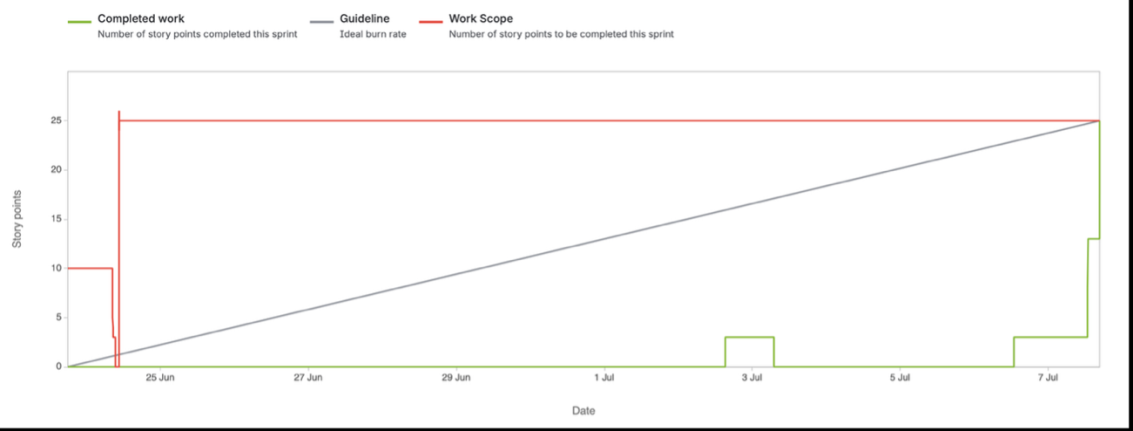
\includegraphics[width=1\linewidth,height=\textheight,keepaspectratio]{assets/sprints/sprint5-burndown.png}
\caption{Sprint 5 burnup chart (Jira).}\label{fig:sprint5-burndown}
\end{figure}

\subsubsection{Final Retrospective}\label{sec:sprint5-retrospective}

Since no next sprint remained to derive action items for, the team replaced the usual retrospective format with a retrospective across the full twelve weeks, held in person on a Miro board built for the occasion (\cref{fig:sprint5-retrospective}). In the team's own assessment, what carried the project were the discipline of sticking to the Scrum plan, the consistently good mood, and the collaboration with Interhyp. What ran less smoothly were coordinating five personal schedules, applying Scrum rigidly to work that was at times research-heavy rather than feature-shaped, and the recurring friction of exhausting LLM token budgets during training runs. The biggest learnings were that a substantial project is achievable within twelve weeks when a team commits to it, that coordinating a university project across individual schedules is harder than coordinating work in a professional context, and that stepping back early beats getting stuck in details. Asked what it would do differently, the team named more open communication from the start, more in-person sessions, and a looser application of Scrum where the work did not call for its full structure. None of this changed the closing sentiment of the session, which was pride in the collaboration and in the product handed over.

\begin{figure}
\centering
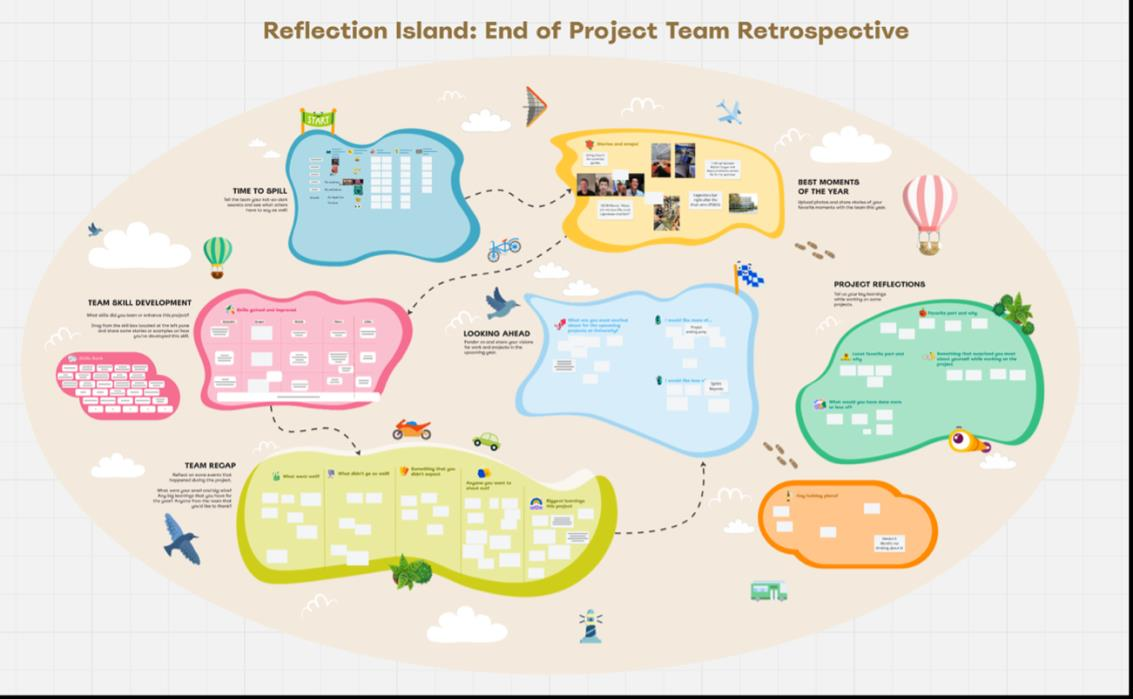
\includegraphics[width=1\linewidth,height=\textheight,keepaspectratio]{assets/sprints/sprint5-retrospective.png}
\caption{Final project retrospective board (Miro).}\label{fig:sprint5-retrospective}
\end{figure}
